\documentclass[10pt,a4paper]{article}
\usepackage[margin=20mm]{geometry}
\usepackage[T1]{fontenc}
\usepackage{lmodern,microtype,graphicx,booktabs,tabularx,xcolor}
\usepackage[hidelinks,pdftitle={Vehicle Rental Database: Technical Brief Report},pdfauthor={}]{hyperref}
\definecolor{ink}{HTML}{123349}
\usepackage{titlesec}
\titleformat{\section}{\large\bfseries\color{ink}}{}{0pt}{}
\titlespacing*{\section}{0pt}{12pt}{5pt}
\setlength{\parindent}{0pt}
\setlength{\parskip}{6pt}
\begin{document}
{\LARGE\bfseries\color{ink} Vehicle Rental Database}\par
{\large Technical Brief Report}\par
{\small HY360 Databases \enspace|\enspace Java, JDBC, MySQL, Servlets}
\vspace{6pt}

A database for a rental service that manages customers, vehicles, rental history, and repair reports. The project connects relational modeling with SQL queries and Java data access. A small web interface exposes part of the implementation.

\section*{Relational design}
The schema contains nine tables. \texttt{Registration} stores account records and \texttt{Customer} holds customer details. \texttt{Vehicle} contains shared attributes such as brand, autonomy, daily costs, and availability. Four category tables add attributes for cars, motorcycles, bicycles, and electric scooters. \texttt{Rental} links a customer to a vehicle for a dated rental, while \texttt{Report} records vehicle faults and repair expenditure.

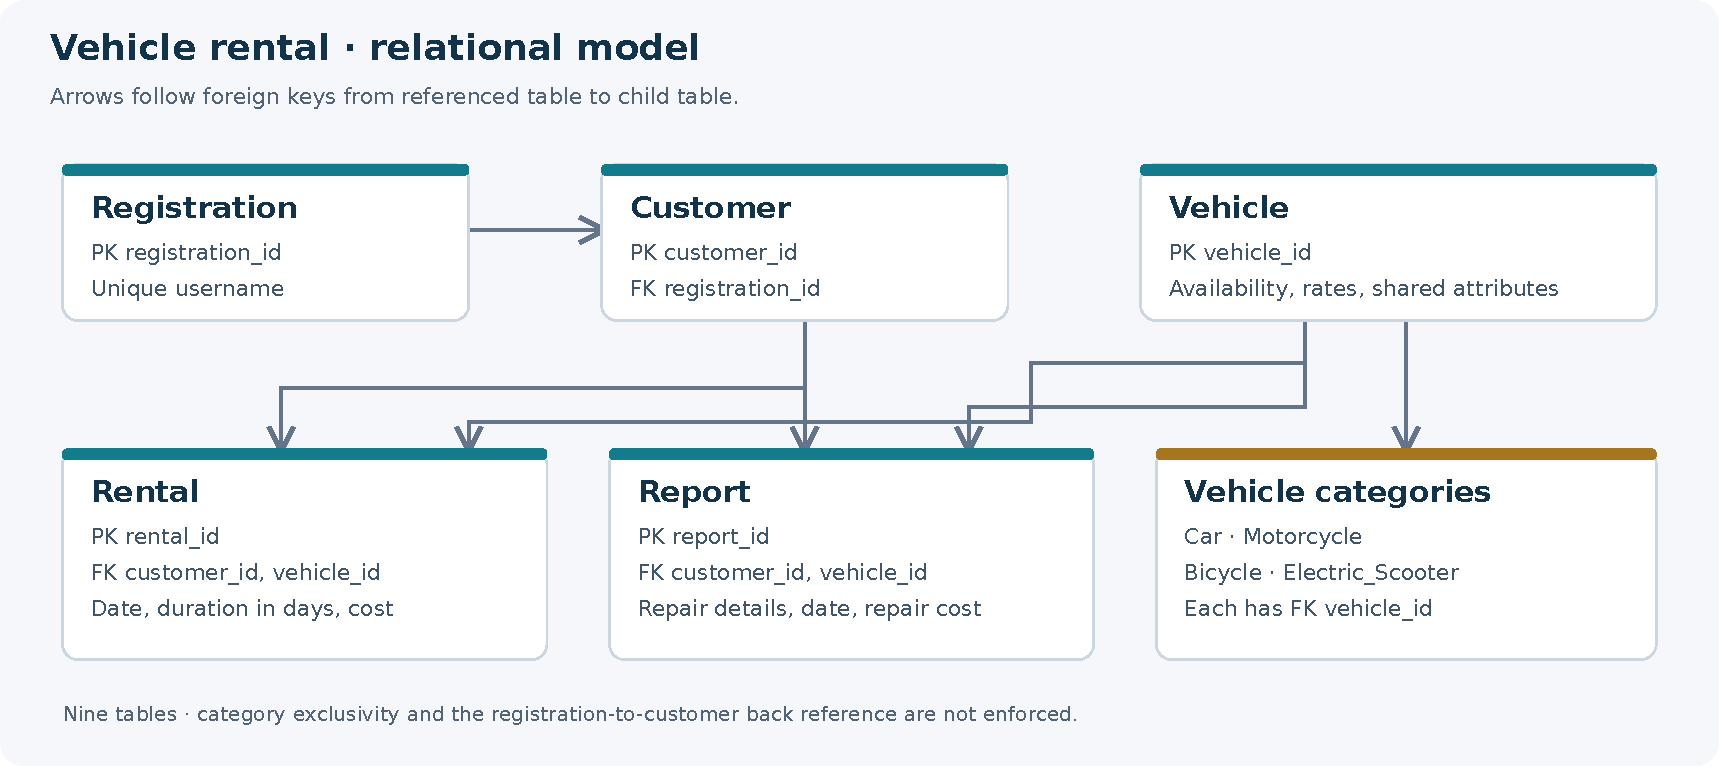
\includegraphics[width=\linewidth]{assets/database-model.pdf}

Foreign keys connect customers to registrations and connect rentals, repairs, and category records to their parent records. Unique constraints protect usernames and selected identifiers. The model separates common vehicle data from category-specific fields, allowing availability and reporting queries to operate on the shared vehicle table.

The constraints have limits. A vehicle can appear in multiple category tables, and \texttt{Registration.customer\_id} has no foreign key back to \texttt{Customer}. Birth dates are represented as integer years, availability as text, and rental costs as integers. These choices keep the course implementation simple but leave validation and richer domain rules to application code.

\section*{Java data access}
Table helpers build the schema and execute JDBC queries. Domain objects represent rows, and Gson supports conversion between query results, JSON, and Java objects. Availability helpers filter category records using the shared vehicle availability field. Servlet endpoints return the resulting data to the browser.

The application is packaged as a Maven WAR using the \texttt{javax.servlet} API. Database settings are supplied through environment variables or JVM properties, so a local MySQL connection can be configured without editing source code. Tomcat 9 matches the servlet namespace used by the project.

\newpage
\section*{SQL reporting}
Five executable queries demonstrate joins, filtering, grouping, and aggregation. The synthetic fixture includes six vehicles across four categories, five rentals spanning two calendar years, and three repair records.

\renewcommand{\arraystretch}{1.25}
\begin{tabularx}{\linewidth}{@{}p{0.25\linewidth}X@{}}
\toprule
Query & Engineering detail \\
\midrule
Inventory & Left joins connect shared vehicle records with category attributes. \\
Period rentals & Customer and vehicle joins enrich rental records within a half-open date interval. \\
Rental duration & Minimum, maximum, and average duration are grouped by rented vehicle. \\
Rental revenue & A left join retains vehicles with no rentals in the selected period. The period predicate stays in the join condition. \\
Repair expenditure & A period filter and aggregate total repair costs, returning zero for an empty result. \\
\bottomrule
\end{tabularx}

Keeping the date condition inside the revenue join matters: moving it to a \texttt{WHERE} clause would discard vehicles without matching rentals. The queries use the stored rental cost rather than recomputing historical charges from current daily rates.

\section*{Verification}
Running \texttt{mvn verify} builds the WAR and executes seven integration tests on an isolated H2 database in MySQL compatibility mode. The tests create tables through the Java builders, apply the same synthetic fixture to the exported SQL schema, check foreign-key and uniqueness rejection, and exercise three availability helpers and all five reports.

The 2024 fixture produces rental revenue of 410 and repair expenditure of 100 in the schema's unspecified monetary units. Vehicle 1 has two rentals lasting two and three days, giving an average of 2.5 days. Revenue output retains all six vehicles, including those with zero revenue in the interval. These are deterministic fixture results, not service or performance measurements.

H2 verification establishes the tested JDBC and SQL behavior. It does not establish MySQL deployment compatibility or complete browser workflows. The setup guide gives separate instructions for a local MySQL database and Tomcat deployment.

\section*{Implementation scope}
The database model, query paths, and Java integration form the core of the project. The web shell has incomplete registration, session restoration, motorcycle routing, and accident submission. Some individual-record helpers also contain malformed SQL or incomplete error handling.

Passwords and payment details are plain fields, and several queries concatenate input. Completing the application would require secure authentication and payment-data design, prepared statements, transaction handling, authorization, and end-to-end workflow checks. Detailed implementation boundaries and reproduction instructions are in \texttt{docs/SETUP.md}.

\vfill
{\small\color{ink}\url{https://github.com/mitsosasim/database}}
\end{document}
